\documentclass[article]{jss}
\usepackage[utf8]{inputenc}

\providecommand{\tightlist}{%
  \setlength{\itemsep}{0pt}\setlength{\parskip}{0pt}}

\author{
Earo Wang\\Monash University \And Di Cook\\Monash Univeristy \And Rob J Hyndman\\Monash Univeristy
}
\title{Calendar-based graphics for visualising people's daily schedules}

\Plainauthor{Earo Wang, Di Cook, Rob J Hyndman}
\Plaintitle{Calendar-based graphics for visualising people's daily schedules}

\Abstract{
It is challenging to visualise people's daily schedules as such data are
often of multiple seasons and of long time span. One example is
Melbourne pedestrian sensor data which are collected at hourly interval
and at a number of locations. Owing to human-related activities, the
primary depiction of the data features multiple temopral scales such as
time of day, day of week, day of year. We develop the
\code{frame\_calendar} function that provides a method for rearranging
such kind of data in a calendar-based format and accomplishing
visualisation with the grammar of graphics, and describe its
construction in detail. We provide some examples to demonstrate its
usage by applying to the pedetrian data.
}

\Keywords{calendar-based visualisation, temporal-context data}
\Plainkeywords{calendar-based visualisation, temporal-context data}

%% publication information
%% \Volume{50}
%% \Issue{9}
%% \Month{June}
%% \Year{2012}
%% \Submitdate{}
%% \Acceptdate{2012-06-04}

\Address{
    Earo Wang\\
  Monash University\\
  Department of Econometrics and Business Statistics, Monash University,
  VIC 3800 Australia\\
  E-mail: \email{earo.wang@monash.edu}\\
  
      Di Cook\\
  Monash Univeristy\\
  Department of Econometrics and Business Statistics, Monash University,
  VIC 3800 Australia\\
  E-mail: \email{dicook@monash.edu}\\
  
      Rob J Hyndman\\
  Monash Univeristy\\
  Department of Econometrics and Business Statistics, Monash University,
  VIC 3800 Australia\\
  E-mail: \email{rob.hyndman@monash.edu}\\
  
  }

% Pandoc header

\usepackage{amsmath}

\begin{document}

\section{Introduction}\label{introduction}

This work was originally motivated by studying foot traffic in the city
of Melbourne \citep{ped}. There have been 43 installed sensors counting
pedestrians every hour across downtown Melbourne until recently. The
dataset can shed lights into understanding people's daily schedules, or
assisting administration and business planning. (FIGURE ?: weekday at
multiple sensors) Figure (?) lends itself to a number of issues that
make exploratory data visualisation challenging in many temporal-context
applications involving human behaviours:

\begin{enumerate}
\def\labelenumi{\arabic{enumi}.}
\tightlist
\item
  Variations primarily result from multiple time scales including time
  of day, day of week, and day of year (such as public holiday and
  recurred events).
\item
  Since the data are often collected at daily frequency or a time scale
  more frequent than daily, they typically involve a large number of
  observations spanning over a long time period.
\item
  Measurements of a single type are made at multiple locations at a
  given time point, which creates a need in comparing and contrasting
  between locations.
\end{enumerate}

Calendar-based graphics turn out to be a useful tool in unfolding
human-related activities in temporal context (cite). For example,
\citet{VanWijkCluster1999} developed a calendar view of heatmap to
represent the number of employees in the work place over a year, where
colours indicate different clusters derived from the days. It remarkably
contrasts weekdays and weekends, highlights public holiday, and presents
other known seasons like school vacations, all of which have influence
over the turn-outs in the office. The calendar-based heatmap was
implemented in a couple of R packages: \pkg{ggTimeSeries}
\citep{R-ggTimeSeries} and \pkg{ggcal} \citep{R-ggcal}. However, these
techniques are too constrained to colour-encoding graphics and day of
week considered as the smallest time window. Time of day, which serves
as one of the most important aspect in explaining variations arising
from pedestrian sensor data, will be neglected through daily
aggregation. Additionally if simply using colours encoded as quantities,
it may becomes less perceivable of the actual variations or behaviours
from the viewer's perspective.

We propose a new algorithm via linear algebra tools to go beyond the
calendar-based heatmap. The approach is developed with these conditions
in mind: (1) to make time of day present in addition to the existing
temporal components such as day of week and day of year, (2) to add line
graphs along with other types of glyphs to the visual toolkit, (3) to
enable an overlaying plot consisting of multiple time series. The
proposed algorithm has been implemented as the \code{frame_calendar}
function in the \pkg{sugrrants} package \citep{R-sugrrants} using
\proglang{R} \citep{R-base}.

The remainder of the paper is organised as follows. Section
\ref{sec:algorithm} describes the \code{frame_calendar} function and the
detailed construction. Section \ref{sec:examples} presents some examples
of its usage. Section \ref{sec:discussion} discusses the advantages and
disadvantages of the method.

\section{Construction}\label{construction}

\label{sec:algorithm}

In the section, the algorithms to construct calendar grids, different
scales, and reference lines and labels are discussed in detail.

\begin{verbatim}
frame_calendar(
  data, x, y, date, calendar = "monthly", dir = "h", sunday = FALSE, 
  nrow = NULL, ncol = NULL, polar = FALSE, scale = "fixed"
)
\end{verbatim}

\subsection{Grid construction}\label{grid-construction}

The algorithm for constructing a calendar plot uses linear algebra,
similar to that used in the glyph map displays for spatio-temporal data
\citep{Wickham2012glyph}. To make a year long calendar, requires cells
for days, embedded in blocks corresponding to months, organised into a
grid layout for a year. Each month can be captured with 35 (5 \(\times\)
7) cells, where the top left is Monday of week 1, and the bottom right
is Sunday of week 5. These cells provide a micro canvas on which to plot
the data. The first day of the month could be any of Monday-Sunday,
which is determined by the year of the calendar. Months are of different
length days, ranging form 28-31, and each month could extend over six
weeks but the convention in these months is to wrap the last few days up
to the top row of the block. The notation for creating these cells is as
follows:

\begin{itemize}
\tightlist
\item
  \(k = 1, \dots , 7\) is the day of the week that is the first day of
  the month.
\item
  \(d = 28, 29, 30\) or \(31\) representing the number of days in any
  month.
\item
  \((i, j)\) is the grid position where \(1 \le i \le 5\) is week within
  the month, \(1 \le j \le 7\), is day of the week.
\item
  \(g = k, \dots,(k+d)\) indexes the day in the month, inside the 35
  possible cells.
\end{itemize}

The grid position for any day in the month is given by

\begin{equation}
  \begin{aligned}
  i &= \lceil (g \mod 35) / 7\rceil, \\
  j &= g \mod 7. \label{eq:grid}
  \end{aligned}
\end{equation}

Figure \ref{fig:month-diagram} illustrates this \((i,j)\) layout for a
month where \(k=5\).

\begin{CodeChunk}
\begin{figure}

{\centering 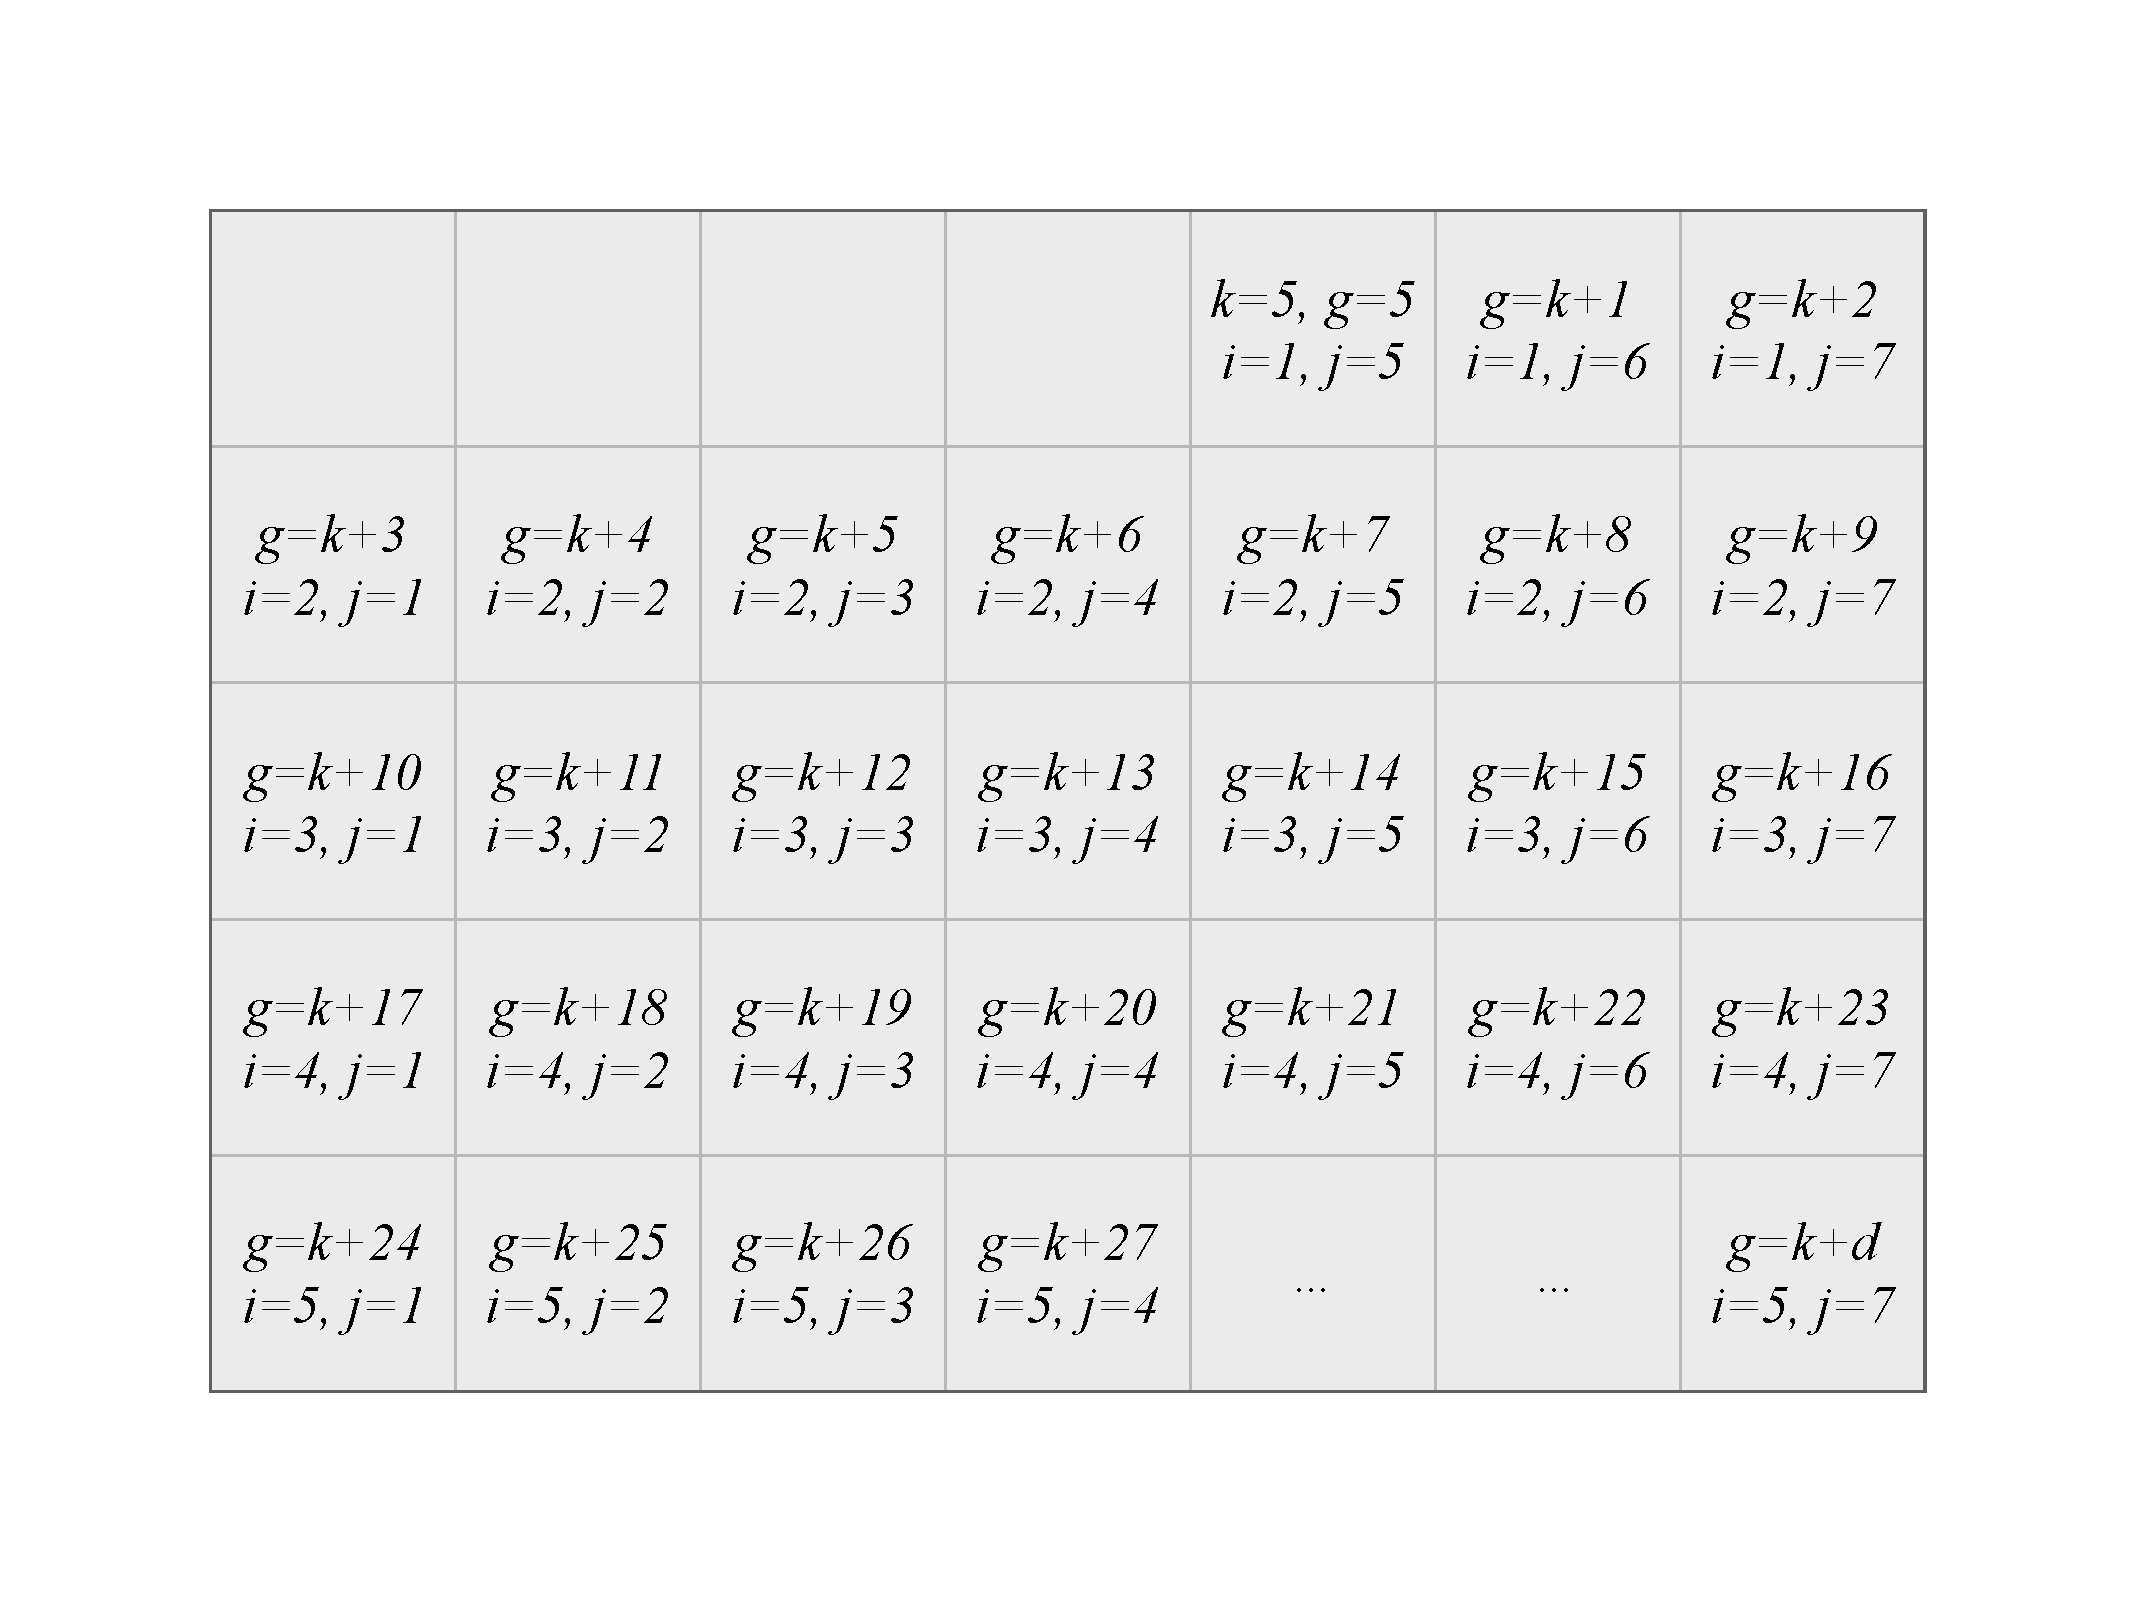
\includegraphics[width=360pt,height=250pt]{figure/month} 

}

\caption[Illustration of the indexing layout for cells in a month]{Illustration of the indexing layout for cells in a month.}\label{fig:month-diagram}
\end{figure}
\end{CodeChunk}

To create the layout for a full year, \((m, n)\) denotes the position of
the month arranged in the plot, where \(1 \le m \le M\) and
\(1 \le n \le N\). Between each month requires some small amount of
white space, label this \(b\). Figure \ref{fig:year-diagram} illustrates
this layout.

\begin{CodeChunk}
\begin{figure}

{\centering 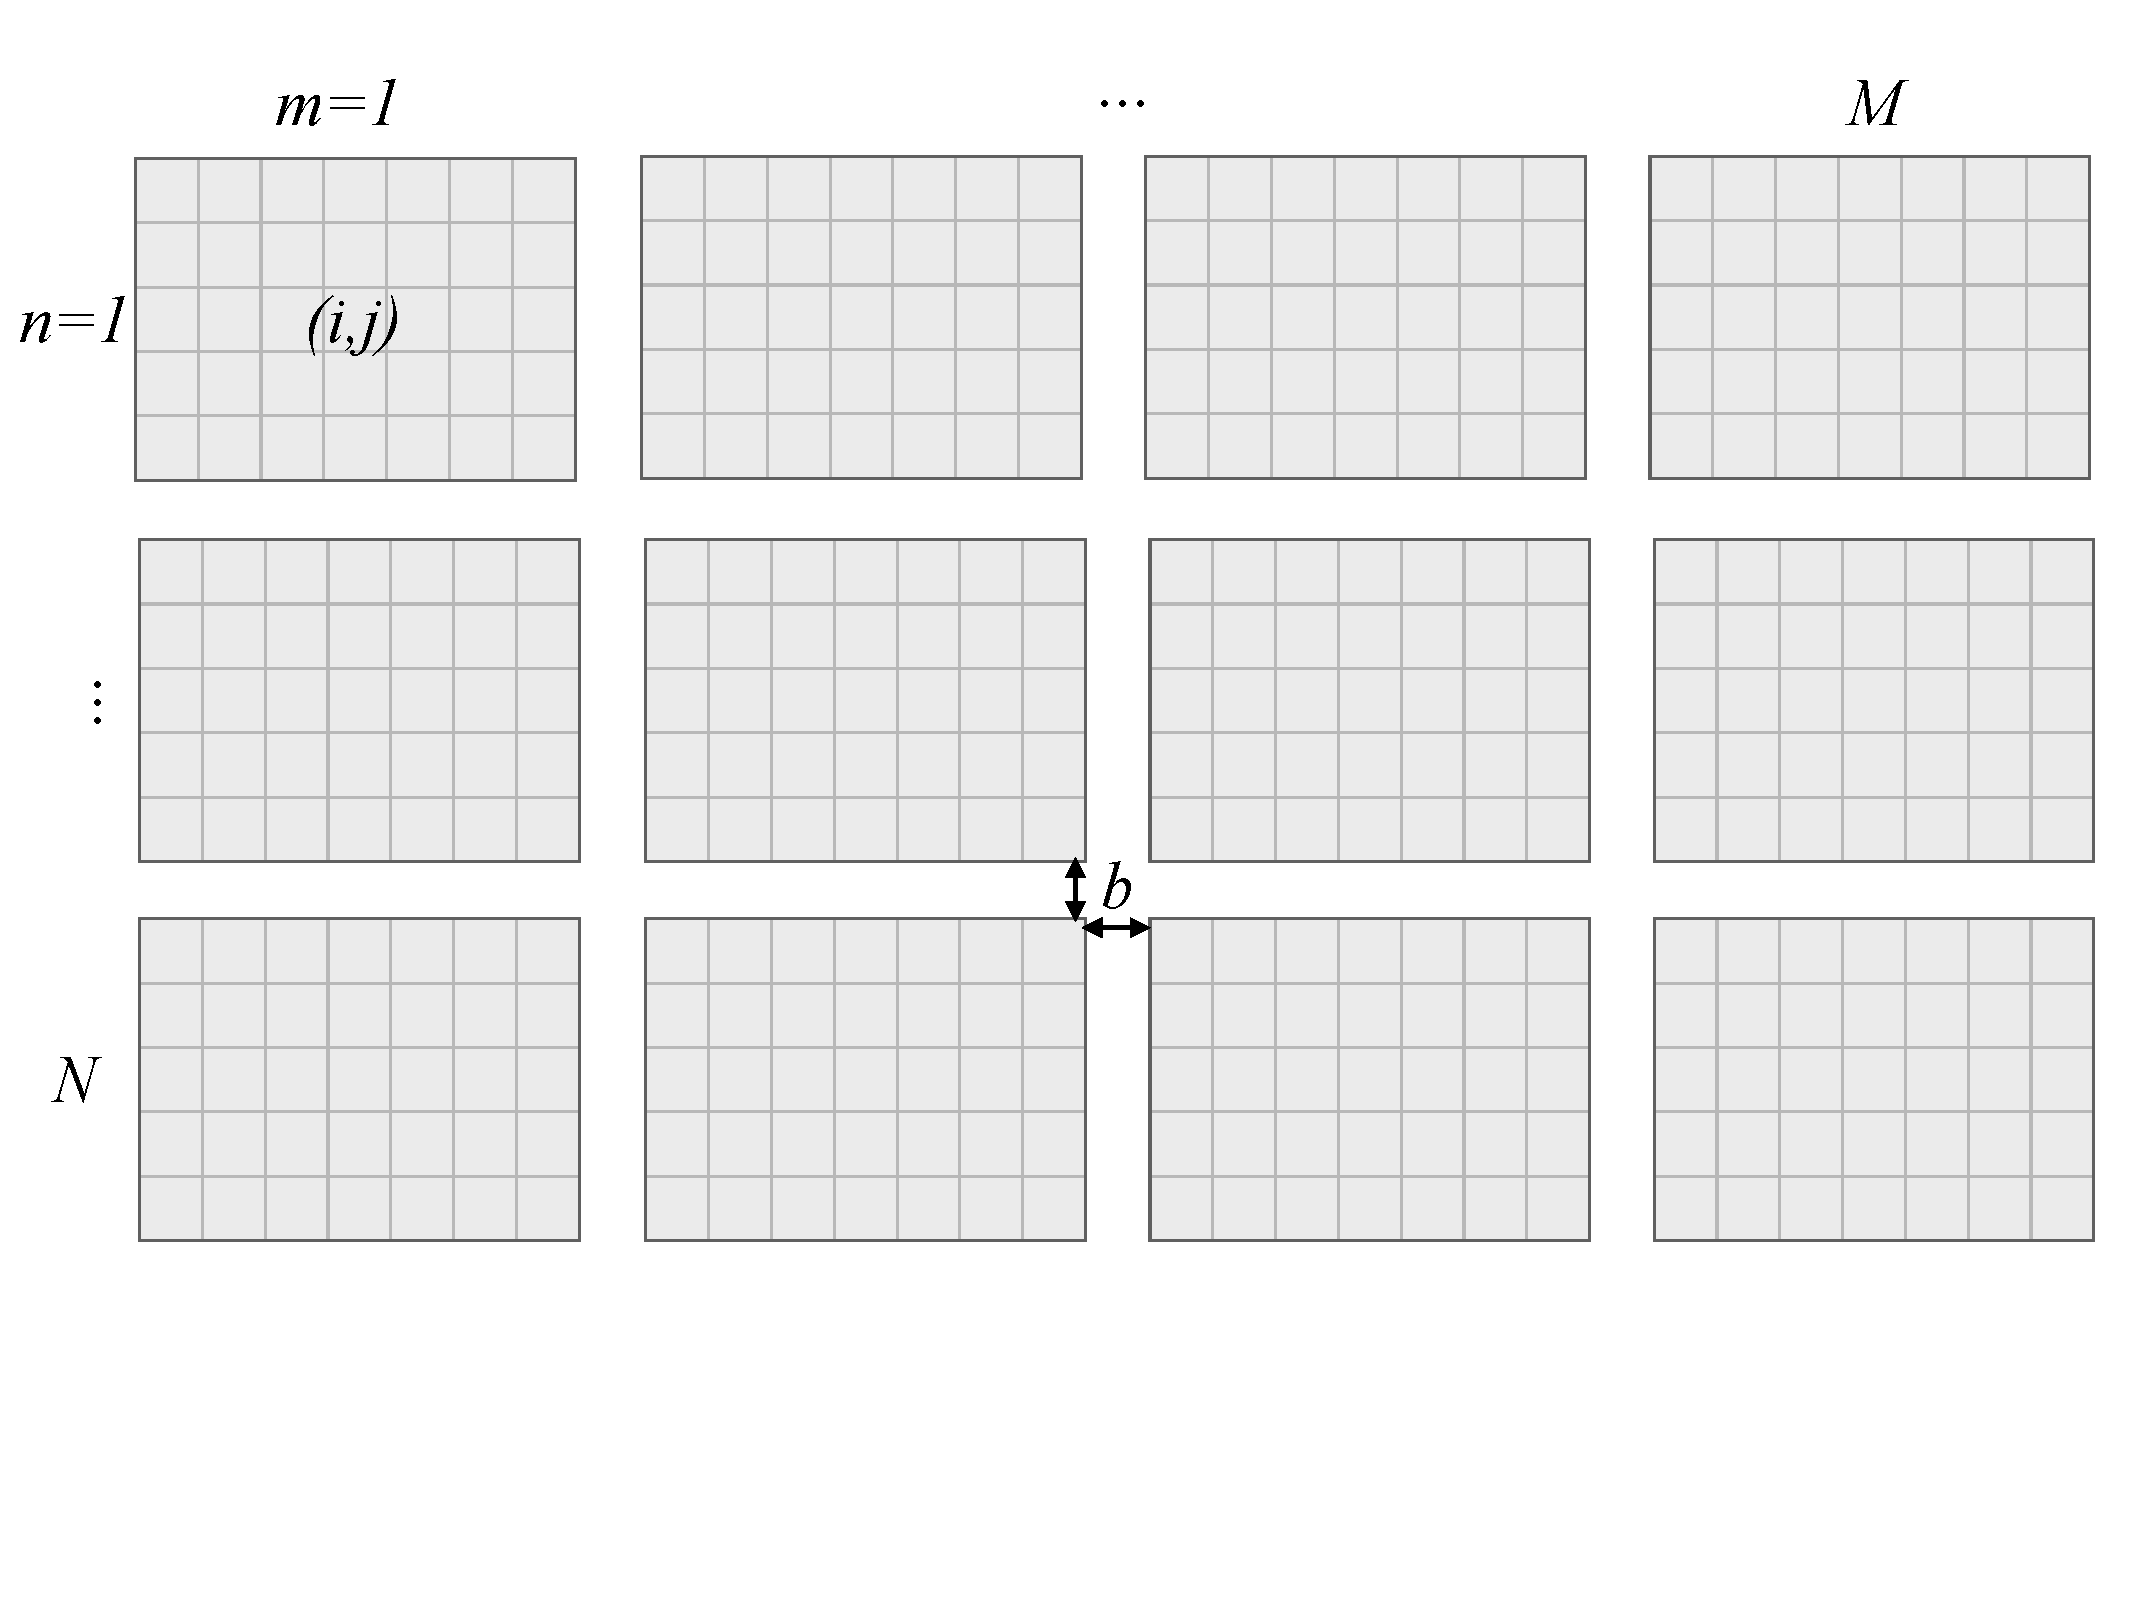
\includegraphics[width=360pt,height=250pt]{figure/year} 

}

\caption[Illustration of the indexing layout for months of one year]{Illustration of the indexing layout for months of one year.}\label{fig:year-diagram}
\end{figure}
\end{CodeChunk}

Each cell forms a canvas on which to draw the data. Consider the canvas
to have limits \([0, 1]\) horizontally and vertically. For the
pedestrian sensor data, within each cell hour is plotted horizontally
and count is plotted vertically. Each variable is scaled to have values
between \([0,1]\), using the minimum and maximum of all the data values
to be displayed assuming of fixed scales. Let \(h\) be the scaled hour,
and \(c\) the scaled count.

Then the final points for making the calendar line plots of the
pedestrian sensor data is given by:

\begin{equation}
  \begin{aligned}
  x &= i + (i - 1) \times m + (m - 1) \times b + h, \\
  y &= -j - (j - 1) \times n - (n - 1) \times b + c. \label{eq:final}
  \end{aligned}
\end{equation}

Note that for the vertical direction, the top left is the starting point
of the grid, hence the subtractions, and resulting negative values to
lay out the cells. Within each cell, the starting position is bottom
left.

The algorithm can be relatively easily extended to layout from a single
month to a few years, based on the period of time to be visualised.
\((M, N)\) can be determined by the user using the arguments of
\code{nrow} and \code{ncol}. If the one would like to visualise data
spanning over three years, for example, \(M = 12\) and \(N = 3\) seem to
be an appropriate choice when assessing the differences of a given month
across the years.

The algorithm can be simplified to accommodate the other two types of
calendar formats. One is comprised of days of a week in columns and
weeks of a year in rows, and the other is days of a month in columns and
months of a year in rows, which we refer to as ``weekly'' and ``daily''
calendar respectively. Due to the arrangements, the weekly calendar puts
more emphases on days of a week over days of a year, whereas the daily
one serves as the opposite. The monthly format can be considered as the
advanced twist of both weekly and daily. Temporal patterns lead to which
format to be employed. The weekly calendar can be a nice attempt if the
most variations can be characterised by days of a week. On the other
hand, the absence of weekly effect but the presence of yearly effect can
direct to the daily calendar. When both are present, the monthly
calendar appears to be a better choice.

We only illustrate that grids are laid out over the horizontal direction
in the paper. The vertical direction can be enabled by swapping \(i\)
and \(j\) in the algorithm stated above. It is particularly useful for
those users who get accustomed to calendars of vertical organisation in
some countries.

\subsection{Scales}\label{scales}

One of the advantages using glyphs over heatmaps is evident in easily
enabling scales on different temporal scales. All of the line glyphs
shown above are drawn on the global scale so that it makes the
magnitudes comparable over all the period. On the other hand, some
sub-series of small magnitudes yet worth-noting shapes possibly become
invisible whilst embedded in the overall picture. The individual scale
or something else, as a result, complements the calendar-based
visualisation in general.

There are other three types of scales in addition to the global scale:
individual scales regardless of days, conditional on weekdays, and
conditional on days of a month.

\subsection{Reference lines and
labels}\label{reference-lines-and-labels}

It can be noted that reference lines separating each cell and panel and
labels indicating weekday and month are also constructed in order to
make calendar-based graphics more accessible and informative.

Regarding the monthly calendar format, the major reference lines
separate every month panel and the minor ones separate every day cell,
represented by the think and thin lines respectively. The major
reference lines are placed on the far left and right as well as the
bottom and top of every month panel: for each \(m\), the vertical lines
are determined by \(\min{(x)}\) and \(\max{(x)}\); for each \(n\), the
horizontal lines are computed by \(\min{(y)}\) and \(\max{(y)}\). The
minor reference lines are placed on the initial positions: for each
\(i\), the vertical line is \(\min{(x)}\); for each \(j\), the
horizontal line is \(\min{(y)}\).

The abbreviated month labels located on the top left are obtained
through \((\min{(x)}, \max{(y)})\) for every \(m\) and \(n\). The
weekday texts with a single letter are uniformly placed on the bottom of
the whole canvas, that is \(\min{(y)}\).

\section{Examples}\label{examples}

\label{sec:examples}

\section{Discussion}\label{discussion}

\label{sec:discussion}

The calendar-based visualisation provides data plots in the familiar (at
least for the Western world) format of an everyday tool. Special events
for the region, like Anzac Day in Australia, or Thanksgiving Day in the
USA, more easily pop out to the viewer as public holidays, rather than a
typical work day.

This sort of layout may be useful for studying consumer trends, or human
behaviour, like the pedestrian patterns. It may not work so well for
physical patterns like temperature, which are not typically affected by
human activity.

The limitation is also evident: hard to perceive trend as not on the
common scale.

We shall enable interactivity in the calendar-based graphics for time
series data. It will allow users to transform different temporal
components and switch displays between overlaying and faceting through
key strokes or mouse clicks.

\bibliography{packages.bib,references.bib}


\end{document}

